\documentclass[a4paper,10pt,oneside]{scrreprt}
\usepackage[latin1]{inputenc}
\usepackage[english]{babel}
\usepackage{graphicx}
\usepackage{float}
\usepackage{geometry}
\geometry{verbose,a4paper,tmargin=15mm,bmargin=25mm,lmargin=15mm,rmargin=15mm}
\usepackage{paralist}

\usepackage{paracol}

\usepackage{todonotes}

\usepackage{listings}
\lstset{language=Java,
	tabsize=2,
	showspaces=false,
	showtabs=false,
	breaklines=true,
	showstringspaces=false,
	breakatwhitespace=true,
	commentstyle=\color{pgreen},
	keywordstyle=\color{pblue},
	stringstyle=\color{pred},
	basicstyle=\footnotesize\ttfamily,
	moredelim=[il][\textcolor{pgrey}]{$$},
	moredelim=[is][\textcolor{pgrey}]{\%\%}{\%\%}
}

\usepackage{tikz}
\usetikzlibrary{calc,patterns,angles,quotes}

\usepackage{caption}
\usepackage{subcaption}
\usepackage{tabularx} % in the preamble

\usepackage{pdfpages}

%\usepackage{indentfirst} % for always indenting the first paragraphs

\usepackage{wrapfig}
\usepackage{lipsum}
\usepackage[linewidth=1.2pt,linecolor=red]{mdframed} % for boxes around wrapfigure and text

\usepackage{url}

\begin{document}


\begin{center}
	Submitted by Group 18

	\bigskip

	\begin{tabular}{c}
	Group Members: \\
	CETIN, Ulfet (391819); GRUCZKA, FILIP (413279);	LIPINSKI, Bartosz (413177) \\
	SZYMANSKI, Bartosz (411949); GONG, Zeheng (378125)\\
	\end{tabular}

	\bigskip

	DIS1 WS 19/20 - Project Milestone V\\
	Evaluation of Low-Fidelity Prototypes\\

	%	(ordered on lastname basis)
\end{center}
\vspace{-1cm}

\clearpage

% !TEX root = ../Group10_Assignment6_OOSC_2020.tex

\section{Frameworks}

\subsection{Actions Supported}

\begin{itemize}
	\item calculate flat size
	\begin{itemize}
		\item in the current state of SWCArchitect (that is implemented in the previous assignment), we have the 'import floorplan' function. Through that, we can get the information on the imported image, such as width and height.
		\item however, those features of width and height are abstract, they do not map to the real-world information without extra information. Due to this nature of those features, we can either:
		\begin{itemize}
			\item provide flat size in pixel$^{2}$ (e.g. height * width)
			\item we can ask for user intervention, that, at the import of floorplan, we can ask user to provide the dimensions of the flat, so we can map those real world values to the pixels. This would help us also in the other functionalities.
		\end{itemize}
		\item in the previous assignment, we have extended ImageTool to build our ImageImporter (for floorplan). This class' implementation can be used to implement this functionality of calculating flat size.
	\end{itemize}
	\bigskip
	
	\item occupied space of elements/free space
	\begin{itemize}
		\item similar to the 'calculate flat size', we can either ask for user intervention for meter$^{2}$ calculation, or even better, ask for room size once. If we have such information, then we have what is the length of each pixel in horizontal and vertical directions. With such information, we can calculate the relative size of the furnitures too.
		\item in the same sense, we implemented furnitures by extending TextAreaFigure, and we can use this to implement the given functionality.
	\end{itemize}
	\bigskip
	
	\item validate constraints, e.g. "a room has at least three connected walls"
	\begin{itemize}
		\item in the previous assignment, we also implemented some of the constraints.\\
		Citing from our own previous assignment:
		
		\begin{addmargin}[4em]{0em}
			\textit{Wall, Door and Window are extending ImageFigure. Also, Door and Window are created by a special
				CreationTool named "CreateInWallElement". It checks that doors and windows are always placed on a
				wall. If not, it intercepts the call of the framework to mousePressed.}
		\end{addmargin}
		
		\item we can use this to enforce some of the constraints. For the rest of the constraints, we would use Template-Hook approach to enable user to add more constraint by coding, if a need is deemed necessary.
	\end{itemize}
	
	\item mass operations (resizing of multiple objects)
	\begin{itemize}
		\item multiple items can be chosen \& resized.\\
			In order to allow grouping, such as:
			\begin{itemize}
				\item only group certain kind of furniture (e.g. only chairs)
				\item group more than one kind of furniture (like the example in the previous assignment: table \& chair grouping)
			\end{itemize}
	
		\item for such flexibility, we would also use one of the Template-Hook approaches, so the user-generated furniture types are also allowed to be grouped without selecting them manually.
	\end{itemize}
\end{itemize}

\subsection{UI choice}

We would like to select the first of the provided UI dialogues. Thanks to the jHotDraw support of the menu implementation, it would allow for an easier and cleaner implementation of the inclusion of additional features. A drop-down added to the menu-bar would also allow for the users to already feel comfortable with functionality that is added in an intuitive way. We believe that the second UI could confuse potential users of our application with regards to the behaviour of the added functionality.

\subsection{Framework properties and patterns}
We would like to define this framework as a white-box framework, as it will be an extension of the jHotDraw framework. We would like to propose an implementation that would allow the usage of elements such as Figures. For that to work nicely, we would like to propose the following patterns to provide support of our implementation:

\subsubsection{Calculate flat size}
For the calculation of the flat area, we would like to propose the usage of \textbf{Singleton Pattern}. We would like to additionally ask the user after they upload a background image to provide the width and height of the flat. Those could then be mapped onto the amount of pixels in width and height respectively to be able to approximate the size of each of the elements. This means that the flat size would be not only an accurate measure, but also easily accessible by all components that need it.

\subsubsection{Occupied space of elements/free space}
The calculation of the occupied space/free space would also follow a similar set of steps as the flat size, but due to various object types usage, we would like to use the \textbf{Template Method Pattern}. This would allow us to provide an abstract structure containing general methods of concepts, which we could then be made more concrete in the respective classes, which define the calculation of specific object types. The calculation of the occupied space would then simply be made by addition of the results of the helper classes. One could then obtain the free space based on the subtraction between the flat size and the above mentioned addition result.

\subsubsection{Validate constraints}
For the validation of constraints we would like to propose the \textbf{1:n Connection meta-pattern} with \textbf{Observer pattern}. Not only would we then be able to define constraints for various types of objects, but also provide a quick response to the changes made in the UI by the user. This is very important in the constraint validation. As we have various object types and various constraints that are relevant to them, the 1:n Connection seems a relatively obvious choice.
The notify in the ConstraintHolder would then be responsible for keeping track of all elements, which are managed in terms of a specific type of constraints and notifying all relevant observers if a constraint violation has been detected. ConstraintHolder contains also a list of all constraints to help in the notify process.

\subsubsection{Mass operations}
We would like to propose the usage of event listeners in each of the objects. When the user would like to for example resize all chairs in the image, they would have to emit chair resize event, which would trigger all relevant chairs to update their sizing accordingly.


\subsection{UML Diagrams}

\subsubsection{Area Calculations}

\includegraphics[width=\textwidth]{../uml/area}

\subsubsection{Constraint Validation}

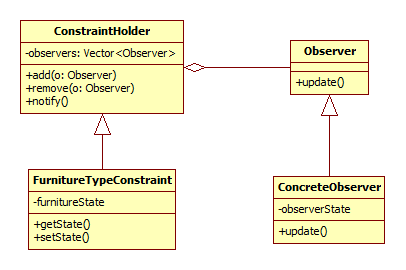
\includegraphics[width=\textwidth]{../uml/constraint.png}


\section{Solution \#2}

\subsection{Objective of the study}
To find whether our prototype about Shopping Companion would be well-received or not



\subsection{Contextual Information}
the experiment held in a hall in Computer Engineering Department of RWTH. There were passerby people, which we cannot avoid. This might have created tension on the user, yet it was our best call.


\subsection{Details of the task}
The Model Extraction is employed to extract what user understand from the prototype. In addition, this prototype employs a genie, who can talk and direct the user. In order to emulate that with our low budget, I played the role of the genie. (I only read the text on the interface, and did not add any other word in my speech to the users)

\subsection{Experimental Procedure}

\begin{itemize}
	\item User is greeted, and her consent is openly asked.
	\item The items on the left (items from a supermarket) are explained, that they are actual items from supermarket and they are emulating supermarket aisles.
	\item The prototype is explained briefly, that the paper belongs to the application UI and how one can interact with that.
	\item Pre-provided cellphone with a shopping list on it is explained to the user.
	\item The user synchronizes using the given phone.
	\item The shopping list appears on the tablet, and the genie encourages user to start scanning items.
	\item The user scans the shopping items on her left in any order she wants.
		\begin{itemize}
			\item whenever an item is scanned, an appropriate UI change (information about the scanned item, crossing out the item from the shopping list, advice on health) has been made.
		\end{itemize}
	\item as the shopping list is depleted, the user is informed about this event and asked whether she wants to continue shopping. In case the user wants to continue, UI goes back to displaying shopping list and is ready to start upcoming items, if there is any.
\end{itemize}

\subsection{Unedited video}
Please see the following YouTube links
\begin{itemize}
	\item Tina
		\begin{itemize}
			\item UI and user interaction videos, merged side-by-side into one: \url{videos/shopping companion/tina_test.mp4}
			
			\item the user feedback after the experiment: \url{videos/shopping companion/tina_feedback.mp4}
		\end{itemize}
	
	\item Enes
	\begin{itemize}
		\item UI and user interaction videos, merged side-by-side into one: \url{videos/shopping companion/enes_test.mp4}
		
		\item the user feedback after the experiment: \url{videos/shopping companion/enes_feedback.mp4}
	\end{itemize}
\end{itemize}

\subsection{Important findings}

	\begin{itemize}
		\item Users liked the voice feedback that is provided. (we were not sure about whether to provide voice-over or not, now it is evident that it is beneficial) (was also a tip from our advisor)
		\item the writing style of the comment on unhealthy products are described to be a bit intrusive: it was also said we might improve on the word selection to make user feel at ease \& not feel to be judged.
		\item using different screens for the comment on some of the products misled the user, and required more time from them to interpret. It is better to stick with single same screen for item identification, and provide the comment there, not in a different page.
		\item the page about the shopping list completion rate seemed a bit different, and user tended to continue shopping. In order to aid this, we decided to remove this page altogether and only provide an exclamation mark over the completion percentage in GUI to make the experience more enjoyable.
		\item feedback on the health concern over some items seemed like a bit off by the users. A recommendation on allowing a user to enable/disable the food health comments is made, which is well-received. On the initial screen, we would provide a switch for user to decide on whether she wants to enable comments on food quality.
	\end{itemize}



\section{Solution \#3}

\subsection{Objective of the study}
To find whether our prototype about Shopping Healthier would be understandable by users and whether users get fun while using this system. Besides, we observe if the users have problems with the usage.

\subsection{Contextual information}
For that is complex to perform the tasks with our low-fidelity prototype in a real supermarket(a supermarket is crowded and we cannot face to emergency scenarios with our low-fi prototype), we have chosen the building of the RWTH Computer Science Falculty to ask our interviewees to perform the tasks.

\subsection{Details of the task}
We use the Model Extraction to see if user have problems with the usage and whether user can  perceive the information from the system well. We ask our interviewees hold our prototype in hand and perform normal shopping process. We show the interaction while the users are shopping without explaning and the user should speak out their thinking of the information they perceived from the prototype. The process takes about 5 to 7 minutes.

\subsection{Experimental procedure}
%Each of the user will follow the same path of the experiment. Before evaluation users will have no idea about out solutions. Additionally we will perform Retrospective Testing.
\begin{itemize}
  \item Initial enviroment setup: we placed the items from the supermarket on the desk to emultate the supermarket enviroment.
  \item Ask the user to do normal shopping process(as in a supermarket).
  \item While the user is shopping items, show the prototype's interaction to the user without explanation.
  \item Ask the user to inform experimenters when the user is done with the whole shopping process to compelete this experimental procedure.
Additionaly, we perform Retrospective Testing.
\end{itemize}


\subsection{Unedited video}
Please see the folder "shopping healthier".
%\subsection{Notes collected during evaluation(optional)}

\subsection{Important findings}
\begin{itemize}
 \item For both users it was unclear at the begining how the redeem procedure and  the "feeding the sheep" system
works. One user suggested to use some kind of pop up message with explanation of the system works.
 \item One of the users liked the idea of choosing her diet, however she noted that more types of diet should be included
 \item Both of the users did enjoy the redeem points system and therefore found this solution fun.
 \item One of the user issue was that he didn't know what exactly to do after he finished shopping. He suggested that there should be a description saying, that user should scan the bardcode afterwards at the check-out.
 \end{itemize}






\end{document}
